
% This LaTeX was auto-generated from MATLAB code.
% To make changes, update the MATLAB code and republish this document.

\documentclass{article}
\usepackage{graphicx}
\usepackage{color}

\sloppy
\definecolor{lightgray}{gray}{0.5}
\setlength{\parindent}{0pt}

\begin{document}

    
    \begin{verbatim}
% Ali Heydari
% Graphing Region of Absolute Convergance
% Math 231 Proj 6
% Reference:
% https://math.boisestate.edu/~wright/courses/m566/StabilityDomains/html/StabilityDomains.html

LW = 'LineWidth'; lw = 1;
N = 1000;
th = linspace(0,2*pi,N);
r = exp(1i*th);

f = @(r) 12*(r.^3-r.^2)./(23*r.^2 - 16*r + 5);
xi = f(r);
plot(xi,'k-',LW,lw),
hold on
fill(real(xi),imag(xi),'c')
x = -1: .2 : 1;
y = x*0;
% plotting the x and y zero lines (axis)
plot(x,y,'k');
plot(y,x,'k');
axis tight
axis equal

title(" Region of Absolute Stability for the Scheme derived in part (a) ");
xlabel("Real Axis");
ylabel("Imaginary");;


hold off
\end{verbatim}

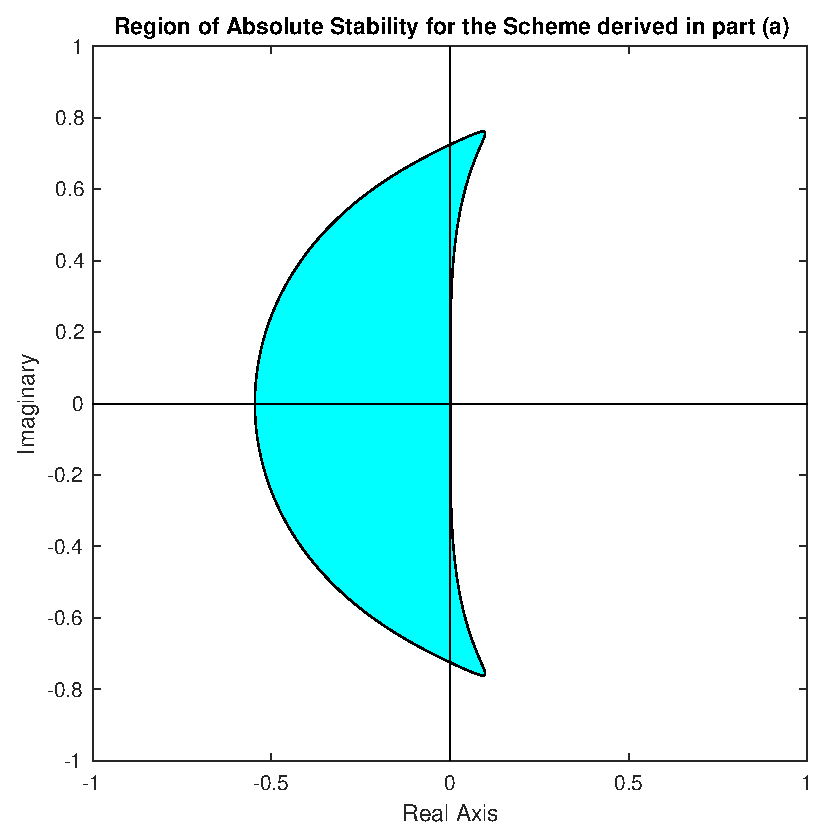
\includegraphics [width=4in]{stability_region_01.eps}



\end{document}
    
